\documentclass[a4paper,11pt]{article}
\usepackage[a4paper, margin=8em]{geometry}

% usa i pacchetti per la scrittura in italiano
\usepackage[french,italian]{babel}
\usepackage[T1]{fontenc}
\usepackage[utf8]{inputenc}
\frenchspacing 

% usa i pacchetti per la formattazione matematica
\usepackage{amsmath, amssymb, amsthm, amsfonts}

% usa altri pacchetti
\usepackage{gensymb}
\usepackage{hyperref}
\usepackage{standalone}

\usepackage{colortbl}

\usepackage{xstring}
\usepackage{karnaugh-map}

% imposta il titolo
\title{Appunti Reti Informatiche}
\author{Luca Seggiani}
\date{2025}

% imposta lo stile
% usa helvetica
\usepackage[scaled]{helvet}
% usa palatino
\usepackage{palatino}
% usa un font monospazio guardabile
\usepackage{lmodern}

\renewcommand{\rmdefault}{ppl}
\renewcommand{\sfdefault}{phv}
\renewcommand{\ttdefault}{lmtt}

% circuiti
\usepackage{circuitikz}
\usetikzlibrary{babel}

% testo cerchiato
\newcommand*\circled[1]{\tikz[baseline=(char.base)]{
            \node[shape=circle,draw,inner sep=2pt] (char) {#1};}}

% disponi il titolo
\makeatletter
\renewcommand{\maketitle} {
	\begin{center} 
		\begin{minipage}[t]{.8\textwidth}
			\textsf{\huge\bfseries \@title} 
		\end{minipage}%
		\begin{minipage}[t]{.2\textwidth}
			\raggedleft \vspace{-1.65em}
			\textsf{\small \@author} \vfill
			\textsf{\small \@date}
		\end{minipage}
		\par
	\end{center}

	\thispagestyle{empty}
	\pagestyle{fancy}
}
\makeatother

% disponi teoremi
\usepackage{tcolorbox}
\newtcolorbox[auto counter, number within=section]{theorem}[2][]{%
	colback=blue!10, 
	colframe=blue!40!black, 
	sharp corners=northwest,
	fonttitle=\sffamily\bfseries, 
	title=Teorema~\thetcbcounter: #2, 
	#1
}

% disponi definizioni
\newtcolorbox[auto counter, number within=section]{definition}[2][]{%
	colback=red!10,
	colframe=red!40!black,
	sharp corners=northwest,
	fonttitle=\sffamily\bfseries,
	title=Definizione~\thetcbcounter: #2,
	#1
}

% disponi codice
\usepackage{listings}
\usepackage[table]{xcolor}

\definecolor{codegreen}{rgb}{0,0.6,0}
\definecolor{codegray}{rgb}{0.5,0.5,0.5}
\definecolor{codepurple}{rgb}{0.58,0,0.82}
\definecolor{backcolour}{rgb}{0.95,0.95,0.92}

\lstdefinestyle{codestyle}{
		backgroundcolor=\color{black!5}, 
		commentstyle=\color{codegreen},
		keywordstyle=\bfseries\color{magenta},
		numberstyle=\sffamily\tiny\color{black!60},
		stringstyle=\color{green!50!black},
		basicstyle=\ttfamily\footnotesize,
		breakatwhitespace=false,         
		breaklines=true,                 
		captionpos=b,                    
		keepspaces=true,                 
		numbers=left,                    
		numbersep=5pt,                  
		showspaces=false,                
		showstringspaces=false,
		showtabs=false,                  
		tabsize=2
}

\lstdefinestyle{shellstyle}{
		backgroundcolor=\color{black!5}, 
		basicstyle=\ttfamily\footnotesize\color{black}, 
		commentstyle=\color{black}, 
		keywordstyle=\color{black},
		numberstyle=\color{black!5},
		stringstyle=\color{black}, 
		showspaces=false,
		showstringspaces=false, 
		showtabs=false, 
		tabsize=2, 
		numbers=none, 
		breaklines=true
}


\lstdefinelanguage{assembler}{ 
  keywords={AAA, AAD, AAM, AAS, ADC, ADCB, ADCW, ADCL, ADD, ADDB, ADDW, ADDL, AND, ANDB, ANDW, ANDL,
        ARPL, BOUND, BSF, BSFL, BSFW, BSR, BSRL, BSRW, BSWAP, BT, BTC, BTCB, BTCW, BTCL, BTR, 
        BTRB, BTRW, BTRL, BTS, BTSB, BTSW, BTSL, CALL, CBW, CDQ, CLC, CLD, CLI, CLTS, CMC, CMP,
        CMPB, CMPW, CMPL, CMPS, CMPSB, CMPSD, CMPSW, CMPXCHG, CMPXCHGB, CMPXCHGW, CMPXCHGL,
        CMPXCHG8B, CPUID, CWDE, DAA, DAS, DEC, DECB, DECW, DECL, DIV, DIVB, DIVW, DIVL, ENTER,
        HLT, IDIV, IDIVB, IDIVW, IDIVL, IMUL, IMULB, IMULW, IMULL, IN, INB, INW, INL, INC, INCB,
        INCW, INCL, INS, INSB, INSD, INSW, INT, INT3, INTO, INVD, INVLPG, IRET, IRETD, JA, JAE,
        JB, JBE, JC, JCXZ, JE, JECXZ, JG, JGE, JL, JLE, JMP, JNA, JNAE, JNB, JNBE, JNC, JNE, JNG,
        JNGE, JNL, JNLE, JNO, JNP, JNS, JNZ, JO, JP, JPE, JPO, JS, JZ, LAHF, LAR, LCALL, LDS,
        LEA, LEAVE, LES, LFS, LGDT, LGS, LIDT, LMSW, LOCK, LODSB, LODSD, LODSW, LOOP, LOOPE,
        LOOPNE, LSL, LSS, LTR, MOV, MOVB, MOVW, MOVL, MOVSB, MOVSD, MOVSW, MOVSX, MOVSXB,
        MOVSXW, MOVSXL, MOVZX, MOVZXB, MOVZXW, MOVZXL, MUL, MULB, MULW, MULL, NEG, NEGB, NEGW,
        NEGL, NOP, NOT, NOTB, NOTW, NOTL, OR, ORB, ORW, ORL, OUT, OUTB, OUTW, OUTL, OUTSB, OUTSD,
        OUTSW, POP, POPL, POPW, POPB, POPA, POPAD, POPF, POPFD, PUSH, PUSHL, PUSHW, PUSHB, PUSHA, 
				PUSHAD, PUSHF, PUSHFD, RCL, RCLB, RCLW, MOVSL, MOVSB, MOVSW, STOSL, STOSB, STOSW, LODSB, LODSW,
				LODSL, INSB, INSW, INSL, OUTSB, OUTSL, OUTSW
        RCLL, RCR, RCRB, RCRW, RCRL, RDMSR, RDPMC, RDTSC, REP, REPE, REPNE, RET, ROL, ROLB, ROLW,
        ROLL, ROR, RORB, RORW, RORL, SAHF, SAL, SALB, SALW, SALL, SAR, SARB, SARW, SARL, SBB,
        SBBB, SBBW, SBBL, SCASB, SCASD, SCASW, SETA, SETAE, SETB, SETBE, SETC, SETE, SETG, SETGE,
        SETL, SETLE, SETNA, SETNAE, SETNB, SETNBE, SETNC, SETNE, SETNG, SETNGE, SETNL, SETNLE,
        SETNO, SETNP, SETNS, SETNZ, SETO, SETP, SETPE, SETPO, SETS, SETZ, SGDT, SHL, SHLB, SHLW,
        SHLL, SHLD, SHR, SHRB, SHRW, SHRL, SHRD, SIDT, SLDT, SMSW, STC, STD, STI, STOSB, STOSD,
        STOSW, STR, SUB, SUBB, SUBW, SUBL, TEST, TESTB, TESTW, TESTL, VERR, VERW, WAIT, WBINVD,
        XADD, XADDB, XADDW, XADDL, XCHG, XCHGB, XCHGW, XCHGL, XLAT, XLATB, XOR, XORB, XORW, XORL},
  keywordstyle=\color{blue}\bfseries,
  ndkeywordstyle=\color{darkgray}\bfseries,
  identifierstyle=\color{black},
  sensitive=false,
  comment=[l]{\#},
  morecomment=[s]{/*}{*/},
  commentstyle=\color{purple}\ttfamily,
  stringstyle=\color{red}\ttfamily,
  morestring=[b]',
  morestring=[b]"
}

\lstset{language=assembler, style=codestyle}

% disponi sezioni
\usepackage{titlesec}

\titleformat{\section}
	{\sffamily\Large\bfseries} 
	{\thesection}{1em}{} 
\titleformat{\subsection}
	{\sffamily\large\bfseries}   
	{\thesubsection}{1em}{} 
\titleformat{\subsubsection}
	{\sffamily\normalsize\bfseries} 
	{\thesubsubsection}{1em}{}

% tikz
\usepackage{tikz}

% float
\usepackage{float}

% grafici
\usepackage{pgfplots}
\pgfplotsset{width=10cm,compat=1.9}

% disponi alberi
\usepackage{forest}

\forestset{
	rectstyle/.style={
		for tree={rectangle,draw,font=\large\sffamily}
	},
	roundstyle/.style={
		for tree={circle,draw,font=\large}
	}
}

% disponi algoritmi
\usepackage{algorithm}
\usepackage{algorithmic}
\makeatletter
\renewcommand{\ALG@name}{Algoritmo}
\makeatother

% disponi numeri di pagina
\usepackage{fancyhdr}
\fancyhf{} 
\fancyfoot[L]{\sffamily{\thepage}}

\makeatletter
\fancyhead[L]{\raisebox{1ex}[0pt][0pt]{\sffamily{\@title \ \@date}}} 
\fancyhead[R]{\raisebox{1ex}[0pt][0pt]{\sffamily{\@author}}}
\makeatother

\begin{document}
% sezione (data)
\section{Lezione del 13-10-25}

% stili pagina
\thispagestyle{empty}
\pagestyle{fancy}

% testo
\subsection{Rilevamento errori}
Il \textit{rilevamento degli errori} (\textbf{error detection}) è il meccanismo attraverso il cui verifichiamo se i dati arrivati attraverso il link fisico sono corretti.

Dobbiamo innanzitutto stabilire un codice di \textbf{rilevamento} degli errori.
Per ogni datagramma trasmettiamo $d$ bit di dati (i bit $D$) e $r$ bit di \textit{rilevamento errore}, o di \textbf{ridondanza} (i bit $R$). Minuscolo è il numero di bit, maiuscolo è il campo di bit vero e proprio.
Sia i bit $D$ che i bit $R$ vengono trasmessi attraverso il link, che ricordiamo è \textit{suscettibile ad errori}.

Per ricavare i bit $R$ si applica una certa funzione $H()$ (sostanzialmente di \textit{hashing}) sui bit $D$. Assunto che mittente e destinatario usino la stessa funzione $H()$, una volta ricevuti i dati il destinatario potrà applicare $H()$ sui bit $D$ ricevuti e ottenere la sua copia dei bit $R$ da confrontare con quelli ricevuti.

Se i bit $R$ corrispondono non ci sono stati errori (a meno della sfortunata circostanza in cui sia i bit $D$ che $R$ sono stati alterati per risultare erroneamente corretti, si sceglie la funzione $H()$ in modo che questo sia difficilmente vero), altrimenti qualcosa è andato storto nella trasmissione sul link.

I bit $R$, nel contesto del \textit{framing} visto in 9.5.1, vengono inseriti nel \textit{trailer} del frame.

\subsubsection{Algoritmi di rilevamento errori}
Vediamo alcune possibili funzioni $H()$ usate per fare rilevamento errori.

\begin{itemize}
	\item \textbf{Parity checking}: posto che si voglia trasferire una parola da $d$ bit: si sceglie un solo bit $R$ di ridondanza, determinato come segue:
		\begin{itemize}
			\item Se il numero di bit a 1 fra i bit $D$ è pari, si imposta il bit in $R$ a 1;
			\item Se il numero di bit a 1 fra i bit $D$ è dispari, si imposta il bit in $R$ a 0.
		\end{itemize}
		In questo caso il bit in $R$ viene detto \textbf{bit di parità} (\textit{parity bit}). Questo algoritmo viene detto di tipo \textbf{even parity}: l'algoritmo opposto si direbbe \textbf{odd parity}.

		Questo algoritmo funziona bene solo nella circostanza in cui il numero di errori sui bit $d$ è dispari (per quanto ci riguarda, 1). Quando si trasferiscono quantità relativamente basse di bit per parola su canali abbastanza affidabili (8, 16, 24 bit su rame o simili) abbiamo che è abbastanza sicuro. Con parole più grandi chiaramente può essere molto più soggetto ad errori.

	\item \textbf{Checksum}: questo sistema, detto della \textit{"somma di controllo"} viene usato in UDP e TCP. 

		In questo caso si prende ogni pacchetto e si divide in blocchi da 16 bit. Sommando questi blocchi bit-a-bit in \textit{complemento a uno} si ottiene un campo $R$ su $r=16$ bit detto \textit{checksum}, che può essere ricalcolato lato destinatario per fare rilevamento degli errori.

		Questo metodo è più sensibile rispetto al bit di parità, e viene usato perlopiù a livello di \textit{trasporto} UDP o TCP (più che a livello \textit{datalink}, dove si fanno altri tipi di controlli meno sensibili).

	\item \textbf{CRC} (\textit{Cyclic Redundancy Check}): questo è il metodo usato più spesso in ambito di \textit{Datalink}.

		Supponiamo di avere $R$ bit dati, e un \textit{pattern} detto \textbf{generatore} $G$ di $r + 1$ bit (dove ricordiamo che $R$ sono i bit di ridondanza e $r$ il loro numero). Mittente e destinatario dovranno entrambi conoscere il generatore.

		Si calcolano quindi il valore dell'operazione $<D, R>$ come:
		$$
		<D, R> = D \times 2^r \  \mathsf{XOR} \  R
		$$
		senza ancora sapere quanto vale $R$. # poco chiaro

		A questo punto il mittente dovrà scegliere i bit $R$ in modo che $<D, R>$ diviso $G$ abbia resto zero: il destinatario potrà quindi calcolarsi $<D, R>$ dai $D$ ed $R$ ottenuti sul link fisico, e noto $G$ effettuare la divisione. Se il resto è diverso da 0, allora si rileva un errore di trasmissione.

		Vediamo come $R$ viene calcolato nella pratica.
		Vogliamo:
		$$
		D \times 2^r \ \mathsf{XOR} \ R = n G \implies D \times 2^r \ \textsf{XOR} \ R
		$$
		per cui $R$ dovrà soddisfare:
		$$
		R = \text{mod}\left( D \times 2^r, G \right)
		$$
		dove \textit{mod} indica il resto della divisione fra i due argomenti (cioè l'operatore modulo).
\end{itemize}

\subsection{Correzione errori}
Dopo aver discusso il \textit{rilevamento degli errori}, vediamo come procedere nella \textbf{correzione degli errori} in caso se ne rilevino.

La soluzione più semplice sarebbe quella di ritrasmettere i datagrammi sbagliati.
Se poi si avesse un algoritmo di rilevamento errori che restituisse esattamente \textit{quali} bit sono errati, basterebbe commutarli per risolvere gli errori.

In questo caso non serve più un codice a \textit{rilevamento} degli errori, ma un codice a \textbf{correzione} degli errori.
Per ogni datagramma trasmettiamo $d$ bit di dati (i bit $D$) e $r$ bit di \textit{correzione errore}, o ancora di \textbf{ridondanza} (i bit $EDC$, da \textit{Error Detection Code}).

Questi sono simmetrici al codice definito per il rilevamento errori: la differenza è che dati $D$ ed $EDC$, lato destinatario possiamo rilevare esattamente l'errore di trasmissione (se c'è stato).

\subsubsection{Algoritmi di correzione errori}
Vediamo alcuni (1) modi per calcolare i bit $EDC$ ed effettuare quindi la correzione degli errori.
\begin{itemize}
	\item \textbf{Parity checking bidimensionale}: si sistemano i bit $D$ in una struttura matriciale, e si calcolano i bit di parità per ogni riga e per ogni colonna. 

		Ad esempio, si può dire:
$$
D = \{ 0, 1, 0, ... \} = \{ d_1, d_2, d_3, ... d_d \} \Rightarrow D_m = 
\begin{pmatrix}
	d_{1,1} & d_{1,2} & ... & d_{1,j} \\ 
	d_{2,1} & d_{2,2} & ... & d_{2,j} \\ 
	... & ... & ... & ... \\
	d_{i,1} & d_{i,2} & ... & d_{i,j} \\ 
\end{pmatrix}
$$
Posti $i$ e $j$ tali che $i \cdot j = d$ (numero di bit in $D$).
A questo punto si orla $D_m$ con i bit di parità di \textit{riga} ($\text{parity}_{row}$) e i bit di parità di \textit{colonna} ($\text{parity}_{row}$):
$$
\begin{pmatrix}
	D_m & \text{parity}_{row} \\
	\text{parity}_{col}
\end{pmatrix}
=
\begin{pmatrix}
\begin{array}{cccc|c}
	d_{1,1} & d_{1,2} & ... & d_{1,j} & d_{1, j + 1} \\ 
	d_{2,1} & d_{2,2} & ... & d_{2,j} & d_{2, j + 1} \\ 
	... & ... & ... & ... & ...\\
	d_{i,1} & d_{i,2} & ... & d_{i,j} & d_{i, j + 1} \\ \hline 
	d_{i + 1, 1} & d_{i + 1, 2} & ... & d_{i + 1, j}  \\ 
\end{array}
\end{pmatrix}
$$
dove
$$
\text{parity}_{row}: \quad d_{r, j + 1} = \text{parity}\left( \sum_{c = 1}^{j} d_{r, c} \right)
$$
$$
\text{parity}_{col}: \quad d_{j + 1, c} = \text{parity}\left( \sum_{r = 1}^{i} d_{r, c} \right)
$$

A questo punto un errore su un singolo $d_{r, c}$ verrà rilevato in quanto incrocierà una riga e una colonna (l'intersezione andrà commutata).
Due o più errori su righe e colonne disgiunte veranno similmente rilevati, a meno di casi di errori multipli su più righe e colonnne (che potrebbero addirittura dare falsi positivi).
Infine, un numero pari di errori sulla stessa riga o sulla stessa colonna ci permettono di rilevare, ma non correggere errori (vedremo 2 colonne sbagliate e una riga giusta, o viceversa, senza poter quindi incrociare).

Chiaramente i bit $EDC$ nel trailer saranno molti di più: per la precisione $i + j$.

\end{itemize}

\subsection{Trasferimento dati}
Abbiamo visto alcuni algoritmi di \textit{rilevamento errori}, introdotto l'ipotesi di effettuare un \textit{reinvio} dei dati corrotti nel caso di errori, e visto anche un algoritmo di \textit{rilevamento e correzione errori}.

Vediamo adesso come realizzare un livello superiore a quello \textit{datalink}, riportando indietro l'ipotesi del reinvio dati, cioè il cosiddetto livello \textit{transfer} o \textbf{trasferimento}, che considereremo un livello \textit{affidabile}.

Le considerazioni che facciamo adesso saranno quelle che nel modello OSI vengono implementate nel cosiddetto livello \textbf{transport}.

L'idea è quella di usare i servizi offerti dal livello datalink per realizzare un'ulteriore astrazione, quella appunto di \textit{trasferimento affidabile}.
\textit{"Confezioneremo"} quindi i pacchetti che vogliamo spedire in datagrammi livello datalink provvisti di un opportuno \textit{header}.

\subsubsection{Primitive di trasferimento}
Per implementare questo tipo di livello \textit{transfer} ci doteremo quindi di alcune primitive a servizio di un'altro \textit{livello superiore}:
\begin{itemize}
	\item \lstinline|rdt_send()|: chiamata dal livello superiore (nella macchina \textit{trasmettitore}), implementa l'invio sul canale affidabile (cioè implementa un protocollo \textbf{RDT} (\textit{Reliable Data Transfer}));
	\item \lstinline|udt_send()|: implementa l'invio sul canale inaffidabile fino al ricevitore;
	\item \lstinline|rdt_rcv()|: implementa il ricevimento sul canale affidabile lato ricevitore, cioè ottiene i dati sul canale inaffidabile, e li corregge (se necessario); 
	\item \lstinline|deliver_data()|: si occupa di inoltrare i dati ottenuti attraverso il protocollo RDT al livello superiore (nella macchina \textit{ricevitore}).
\end{itemize}

Notiamo che le primitive \lstinline|udt_send()| e \lstinline|rdt_recv()| dovranno implementare un qualche tipo di comunicazione bidirezionale (ad esempio se la \lstinline|rdt_rcv()| vuole chiedere il reinvio di un frame perso).

\subsubsection{Macchine a stati finiti}
Per descrivere il protocollo \textbf{RDT} useremo il formalismo della \textit{macchina a stati finiti} (\textbf{FSM}, \textit{Finite State Machine}).

Una macchina a stati finiti rappresenta un \textit{automa} dotato di \textbf{stati} e \textbf{transizioni} fra tali stati: dato uno stato ed un evento si può determinare la transizione successiva, e quindi come si evolve il protocollo. 

\par\smallskip

Nelle prossime sezioni definiremo \textit{iterativamente} versioni sempre più accurate di RDT rispetto a un qualche protocollo reale.

\subsubsection{RDT 1.0}
Iniziamo ad iterare sul nostro protocollo \textit{RDT}.
Assumiamo come prime ipotesi, largamente semplificate:
\begin{itemize}
	\item Non ci sono errori di bit;
	\item Non ci sono perdite di pacchetti. # chiarisci chi è frame, chi è datagramma e chi è pacchetto
\end{itemize}

Prevederemo quindi FSM diverse per \textit{trasmettitore} e \textit{ricevitore}:
\begin{itemize}
	\item Il trasmettitore invia dati su un canale sottostante;
	\item Il ricevitore legge i dat dal canale sottostante.
\end{itemize}

L'FSM in questo caso sarà semplice:
\begin{center}
	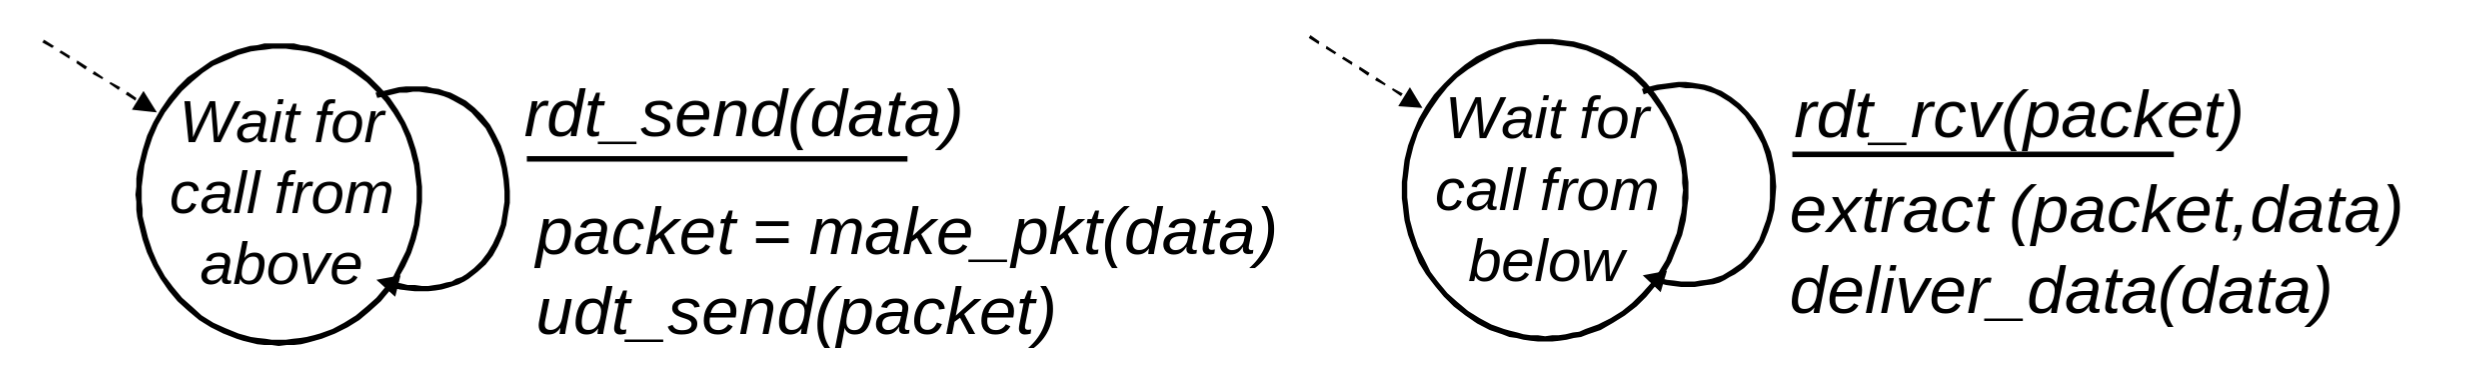
\includegraphics[scale=0.16]{../figures/rdt1fsm.png}
\end{center}
\begin{itemize}
	\item Il trasmettitore avrà il compito di aspettare la chiamata dall'alto, e una volta arrivata di creare un pacchetto da spedire sulla linea inaffidabile;
	\item Il ricevitore avrà il compito di aspettare anch'esso la chiamata dall'alto, e una volta ricevuta mettersi in ascolto per il pacchetto spedito dal trasmettitore. Una volta arrivato, dovrà estrarre i dati dal pacchetto e consegnarli al livello superiore.
\end{itemize}

\subsubsection{RDT 2.0}
Introduciamo un mezzo di trasmissione inaffidabile che potrebbe avere errori di bit, e presumiamo che tale mezzo implementi un qualche livello sottostante (di tipo datalink # datalink maiusc o minusc) che implementa correzione degli errori attraverso CRC o checksum (come visto in 10.1 e 10.2).

Il problema sarà: come riprendersi dagli errori? Abbiamo due modi principali:
\begin{itemize}
	\item \textit{Acknowledgment} (\textbf{ACK}), significa che il ricevitore ha \textit{"capito"}, cioè ha ricevuto il frame correttamente;
	\item \textit{Negative acknowledgment} (\textbf{NAK}), significa che il ricevitor \textit{non ha capito}, cioè non ha ricevuto il frame correttamente.
\end{itemize}

Quando il trasmettitore riceve un \textbf{ACK}, sa di poter procedere con il frame successivo, mentre quando riceve un \textbf{NAK} sa che deve reinviare il frame corrente.

In questo caso l'FSM del trasmettitore ha il seguente aspetto:
\begin{center}
	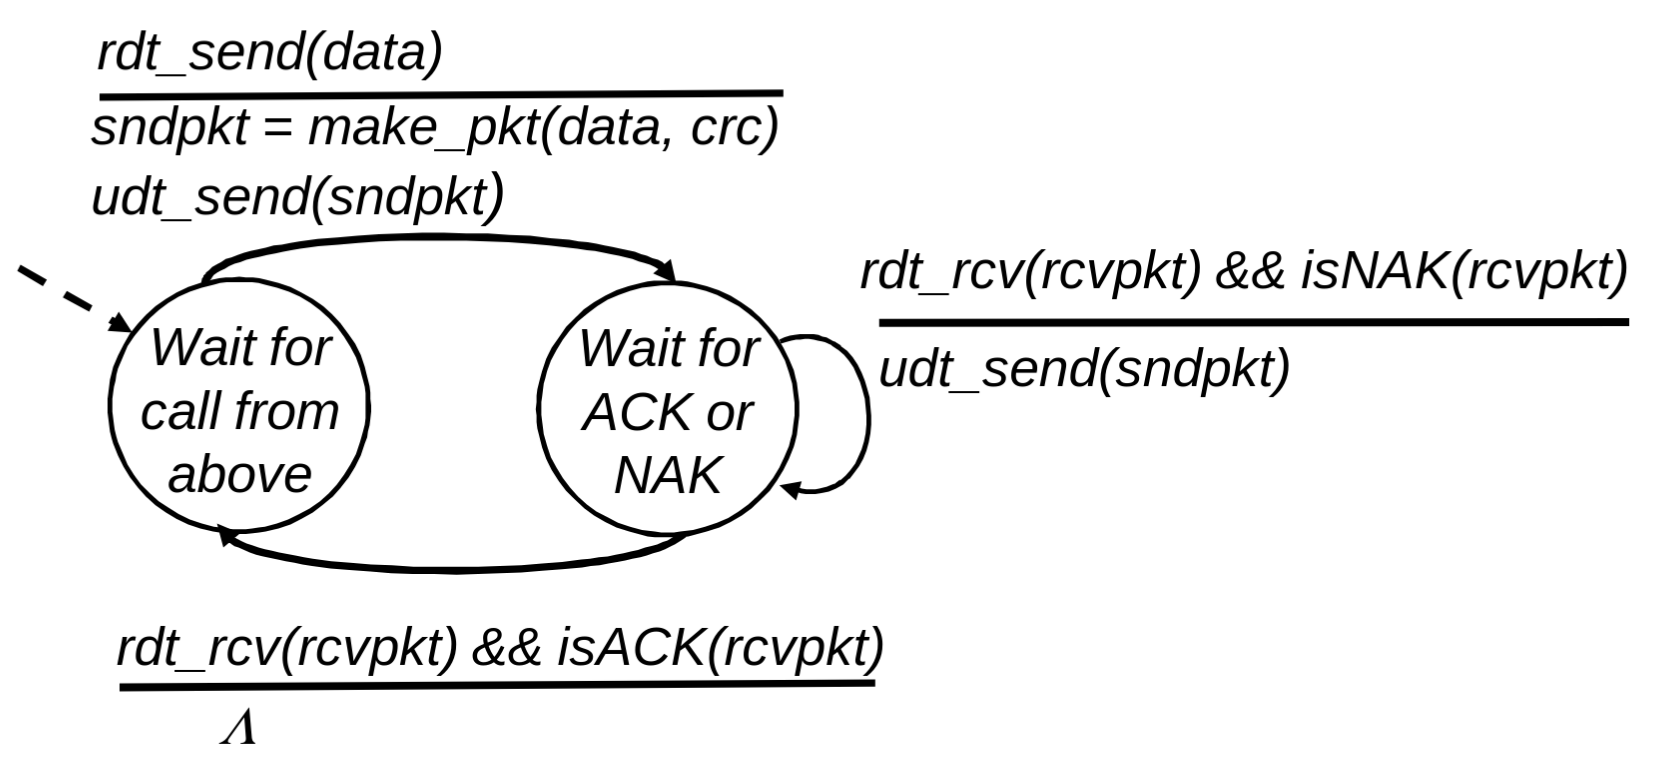
\includegraphics[scale=0.18]{../figures/rdt2fsm.png}
\end{center}
\begin{itemize}
	\item Il trasmettitore avrà il compito, come prima, di aspettare la chiamata dall'alto e quindi inviare il pacchetto sulla linea inaffidabile;
	\item A questo punto dovrà aspettare per un ACK o un NAK dal ricevitore:
		\begin{itemize}
			\item Se riceve un NAK, deve reinviare lo stesso frame;
			\item Altrimenti, cioè se riceve un ACK, deve tornare ad aspettare la chiamata dall'alto per il pacchetto successivo. 
		\end{itemize}
\end{itemize}

Lato ricevitore l'FSM sarà invece:
\begin{center}
	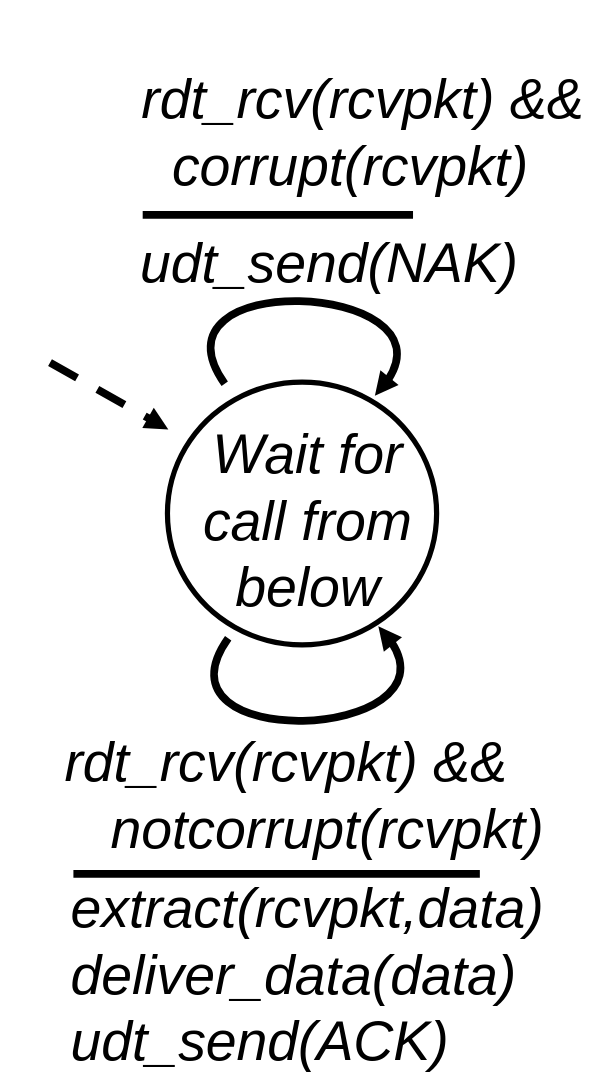
\includegraphics[scale=0.18]{../figures/rdt2fsm2.png}
\end{center}
\begin{itemize}
	\item Il ricevitore dovrà restare in attesa della chiamata dall'alto, e rispondere quindi ai pacchetti ricevuti su linea inaffidabile dal trasmettitore;
	\item Valutata la correzione degli errori sul pacchetto ricevuto, dovrà:
		\begin{itemize}
			\item Inviare il NAK nel caso il pacchetto sia corrotto;
			\item Inviare l'ACK e inoltrare il pacchetto al livello superiore nel caso il pacchetto sia stato ricevuto correttamente.
		\end{itemize}
\end{itemize}


\end{document}
